\documentclass[a4paper,11pt]{report}
\usepackage[T1]{fontenc}
\usepackage[utf8]{inputenc}
\usepackage[polish]{babel}
\usepackage{lmodern}
\usepackage{graphicx}

\title{czas obsługi: stosu, listy}
\author{Tomasz Piotrowski 200524}

\begin{document}
\maketitle

\textbf {\Large{ Sprawozdanie z czasu działania algorytmów  obsługi stosu oraz listy. }}



\begin{figure}
  \begin{center}

  1.Sortowanie liczb ulożonych losowo. Na wykresie widać że dla dużej ilości danych (8mln). Złożoność obliczeniowa wynikająca z wykresu jset wykładnicza. Różnica wynikająca z czasu sortowania w porównaniu do trwania całego procesu jest nieznaczna. Aczkolwiek różnice wraz z przyrostem danych rosną. Piwot obliczany z połowy zbioru powoduje szybszy przyrost czasu działania algorytmu.
  
    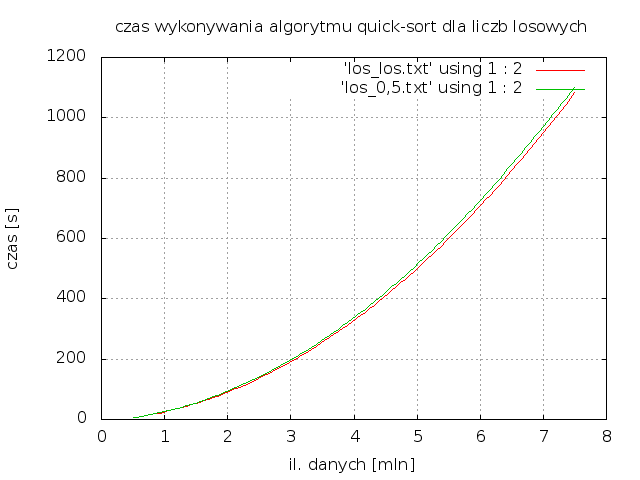
\includegraphics[scale=0.5]{./czas_losowe.png}
    \label{fig:}
    \caption{}
          \begin{tabular}{|l|c|r|}
\hline
il[mln] & czas pół [s] & czas losowo \\
\hline

0.500 & 5.58 & 5.55\\
1.000  &20.75& 20.54\\
1.500  &45.54& 20.54\\
2.000  &82  & 79.17\\
2.500  &127.62& 122.76\\
3.000  &182.67& 175.98\\
3.500  &247.03& 238.5\\
4.000  &321.03&311.73\\
4.500  &401.94&394.04\\
5.000  &494.48&484.67\\
5.500  &612.85&585.61\\
6.000  &708.38&697.49\\
6.500  &838.16&817.87\\
7.000  &973.69&946.64\\
7.500  &1100.37&1082.48\\
\hline
\end{tabular}
\newline
  \end{center}
\end{figure}

\begin{figure}
  \begin{center}
  2. Sortowanie dla zbioru losowego. Przy il danych zbliżonej do 1 mln. Różnica czasowa między piwotem dobieranym losowo a piwotem równym 1/2 zbioru jest niezauważalna. 
    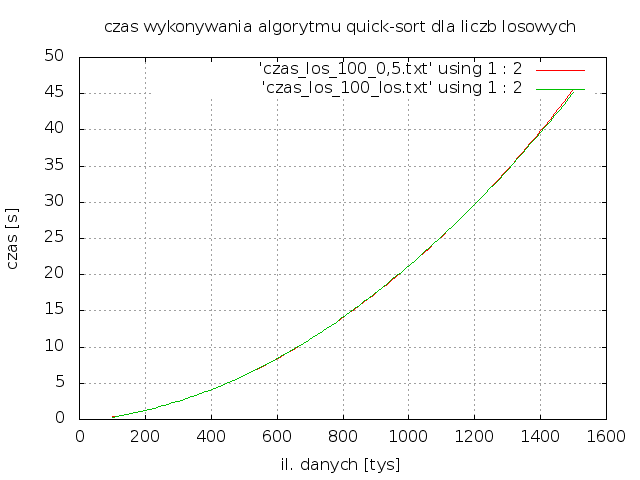
\includegraphics[scale=0.5]{./czas_losowe_100.png}
    \label{fig:}
    \caption{}
          \begin{tabular}{|l|c|r|}
\hline
il[mln] & czas pół [s] & czas losowo \\
\hline

100  & 0.35 & 0.34\\
200  & 1.08 &1.1\\
300  & 2.2 &2.18\\
400  & 3.66 &3.68\\
500  & 5.53 &5.52\\
600  & 7.78 &7.78\\
700  & 10.39 &10.41\\
800  & 13.45 &13.41\\
900  & 16.83 &16.96\\
1000 & 20.59 &20.77\\
1100 & 24.73 &24.78\\
1200 & 29.28 &29.23\\
1300 & 34.2 &34.14\\
1400 & 39.51 &39.48\\
1500 & 45.6 &45.11\\
\hline
\end{tabular}
\newline
  \end{center}
\end{figure}

\begin{figure}

  \begin{center}
 
  3.Sortowanie liczb posortowanych. Wynik pomiarów jest zaskakujący ponieważ dla losowo wybieranego piwotu czas działania algorytmu jest dłuższy niż dla piwotu obliczanego z połowy zbioru.Niestety charakterystyka wciąz wykładnicza.
    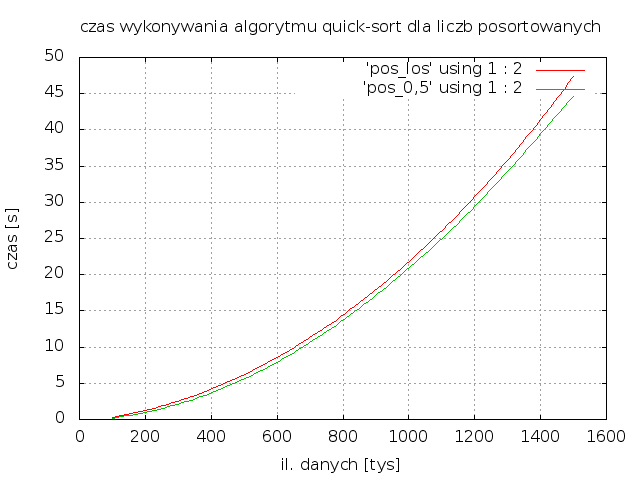
\includegraphics[scale=0.5]{./czas_posortowane.png}
    \label{fig:}
    \caption{}
       \begin{tabular}{|l|c|r|}
\hline
il[mln] & czas pół [s] & czas losowo \\
\hline
100 & 0.205& 0.34\\
200  & 0.795& 1.07\\
300  & 1.79& 2.175\\
400  & 3.15&  3.68\\
500  & 4.94&  5.645\\
600  & 7.105& 8.02\\
700  & 9.925& 10.59\\
800  & 13.415& 13.655\\
900  & 16.52&  17.12\\
1000  & 20.1& 21.205\\
1100  & 24.45& 25.55\\
1200  & 28.945& 30.185\\
1300  & 33.835&  35.295\\
1400  & 39.585& 41.265\\
1500  & 44.64& 47.355\\

\hline
\end{tabular}
\newline
  \end{center}
\end{figure}

\begin{figure}
  \begin{center}
  4. Porównanie wynikow dla 2 omówionych zestawów danych. Liczb posortowanych wcześniej oraz liczb losowych.
    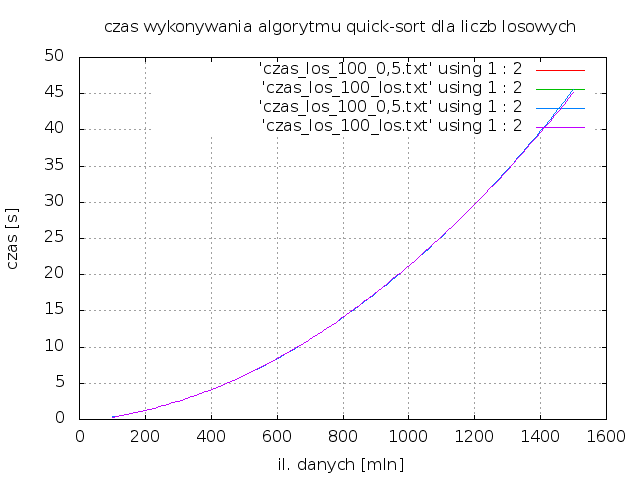
\includegraphics[scale=0.5]{./czas_wszystkie.png}
    \label{fig:}
    \caption{}
          \begin{tabular}{|c|c|}
\hline
dla zbioru losowego & dla zbioru posortowanego \\
\hline

          \begin{tabular}{|l|c|c|c|r|}
\hline
il[mln] & czas pół [s] & czas losowo \\
\hline

100  & 0.35 & 0.34\\
200  & 1.08 &1.1\\
300  & 2.2 &2.18\\
400  & 3.66 &3.68\\
500  & 5.53 &5.52\\
600  & 7.78 &7.78\\
700  & 10.39 &10.41\\
800  & 13.45 &13.41\\
900  & 16.83 &16.96\\
1000 & 20.59 &20.77\\
1100 & 24.73 &24.78\\
1200 & 29.28 &29.23\\
1300 & 34.2 &34.14\\
1400 & 39.51 &39.48\\
1500 & 45.6 &45.11\\
\hline
\end{tabular}
&
       \begin{tabular}{|l|c|r|}
\hline
il[mln] & czas pół [s] & czas losowo \\
\hline
100 & 0.205& 0.34\\
200  & 0.795& 1.07\\
300  & 1.79& 2.175\\
400  & 3.15&  3.68\\
500  & 4.94&  5.645\\
600  & 7.105& 8.02\\
700  & 9.925& 10.59\\
800  & 13.415& 13.655\\
900  & 16.52&  17.12\\
1000  & 20.1& 21.205\\
1100  & 24.45& 25.55\\
1200  & 28.945& 30.185\\
1300  & 33.835&  35.295\\
1400  & 39.585& 41.265\\
1500  & 44.64& 47.355\\

\hline

\end{tabular}
\newline

\end{tabular}
\newline
  \end{center}
\end{figure}
\begin{figure}

\begin{center}


Wnioski \newline
Z pomiarow dokonanych wynika zlozonosc obliczeniowa wykladnicza. Mozliwe ze wpływ na wyniki mają jakieś czynniki związane z systemem operacyjnym, lub błąd w implementacji algorytmu. Z pomiarow mozna wywnioskowac zę dla danych o rozmiarze mniejszym niz 5 mln elementow, różnice czasowe wykonywania algorytmow sa znikome w porownaiu z czasem sortowania.
\end{center}
\end{figure}

\end{document}
